\documentclass[
aps,
pra,
%twocolumn,
showpacs,
preprintnumbers,
amsmath,
amssymb,
footinbib
]{revtex4-2}
\usepackage[breaklinks=true,colorlinks,citecolor=blue,linkcolor=blue,urlcolor=black]{hyperref}
\usepackage{microtype}
\usepackage{bbm}
\usepackage{amsmath}
\usepackage{amssymb}
\usepackage{mathrsfs}
\usepackage{enumitem}		%Item enumeration
%\usepackage{multicol}			%Multi-column formatting
\usepackage{xcolor}			%Adds text coloring commands
\usepackage{graphicx}
\usepackage{multirow}
\usepackage[utf8]{inputenc}
\usepackage{booktabs}
\usepackage[left=2.0cm,top=2.0cm,right=2.0cm,bottom=3cm]{geometry}
\usepackage{fancyhdr}
\usepackage{csquotes}
\usepackage{setspace}
%\usepackage[compact]{titlesec}
\usepackage[normalem]{ulem}

\newcommand*{\req}[1]{Eq.~{\eqref{#1}}}
\newcommand*{\rf}[1]{Fig.~{\ref{#1}}}
\newcommand*{\rsec}[1]{Sect.\,{\ref{#1}}}
\newcommand*{\bb}{\boldsymbol}
\newcommand*{\ar}{{\color{red}ADDREF }}

%\pagestyle{fancyplain}
%\fancyhf{}
%\setlength{\headheight}{15pt}
%\lhead{in preparation}
%\rhead{\today}
%\numberwithin{equation}{section}
%\cfoot{\thepage}
\begin{document}
%\linespread{0.75}
%\thispagestyle{fancy}
%\renewcommand{\abstractname}{}
%\renewcommand{\thefootnote}{\fnsymbol{footnote}}
%\renewcommand\thesection{\Roman{section}}

\title{Mathematical Correspondence Between the Free Fermion and Magnetized Partition Functions}
\author{Andrew Steinmetz}
\email{ajsteinmetz@arizona.edu}
\author{Cheng-Tao Yang}
\author{Johann Rafelski}
\affiliation{Department of Physics, The University of Arizona, Tucson, AZ 85721-0081, USA}
\date{February 17, 2023}

\begin{abstract}
%\begin{spacing}{1.0}
\noindent\textbf{Abstract.} To be written. 
%\end{spacing}
\end{abstract}
\maketitle

\section{Introduction}
\noindent When exposed to external magnetic fields, matter can become magnetized enhancing or reducing the overall net field within the material. The origin of this magnetization is well known to be quantum mechanical in origin. The magnetic susceptibility $\chi$ is a measure of the material response given by
\begin{alignat}{1}
  \label{CHIeq01} \textbf{M}&=\chi\textbf{H}\,,\\
  \label{CHIeq02} \textbf{B}&=\mu_{vac.}\left(\textbf{H}+\textbf{M}\right)=\mu_{vac.}\left(1+\chi\right)\textbf{H}\,,
\end{alignat}
where $\textbf{H}$ is the external magnetic field strength and $\textbf{B}$ is the total magnetic flux density. The magnetization $\textbf{M}$ is the magnetic moment density of the medium. The coefficient $\mu_{vac.}$ is the vacuum permeability, which with $\chi$ can define a material permeability $\mu_{mat.}=\mu_{vac.}(1+\chi)$. Paramagnetism occurs when $\chi>0$ which increases the magnetic flux as the magnetization $\textbf{M}$ is aligned with the external field. In contrast, diamagnetism is when $\chi<0$ reducing the overall magnetic flux as the magnetization is anti-aligned with the external field. In the most general case, the susceptibility can be described by a tensor which is neither paramagnetic or diamagnetic. In this work, we will be considering only the simple case where the susceptibility is single-valued.

Before we handle an ensemble system, we will look at the magnetic moment $\boldsymbol{\mu}$ of a single-particle quantum system. To avoid confusion, the permeability will always be denoted either by a subscript for the vacuum or medium to always differentiate from magnetic moment. If we apply an external field with the local constant value of $B$ which is primarily responsible for the particle's response, the magnetic moment can be evaluated from the matrix element
\begin{alignat}{1}
  \label{CHIeq03} \left|\boldsymbol{\mu}_{n}\right|=-\left\langle n\left|\partial\hat{\mathcal{H}}/\partial B\right|n\right\rangle=-\frac{\partial E_{n}}{\partial B}\,,
\end{alignat}
where $\hat{\mathcal{H}}$ is the Hamiltonian of the system. It is valuable to point out that the individual dipole's response within a medium is only uniquely dependent on the external field $\textbf{H}$ in the case of weak medium magnetization. However, if the bulk magnetization is may easily be large and thus influential to each individual dipole. Physically each dipole is sensitive to the total magnetic flux $\textbf{B}$ which includes a mixture of external field and bulk magnetization $\textbf{M}$ from its neighbors. The magnetization density of the quantum system is then
\begin{alignat}{1}
  \label{CHIeq04} M_{n}(B)=\frac{1}{V}\left|\boldsymbol{\mu}_{n}\right|\,.
\end{alignat}
If we couple the system to a thermal reservoir of temperature $T$, the averaged magnetization at thermal and chemical equilibrium is
\begin{alignat}{1}
  \label{CHIeq05} M(B,T,\eta)=\frac{\sum_{n}M_{n}e^{-\beta (E_{n}-\eta N)}}{\sum_{n}e^{-\beta (E_{n}-\eta N)}}\,,
\end{alignat}
where $\beta=1/k_{B}T$, $k_{B}$ is the Boltzmann constant and $\eta$ is the chemical potential. We then introduce the grand potential $\Phi$ defined by
\begin{alignat}{1}
  \label{CHIeq06} \Phi=-\frac{1}{\beta}\ln\left({\sum_{n}e^{-\beta (E_{n}-\eta N)}}\right)=-\frac{1}{\beta}\ln\left(\mathcal{Z}\right)\,,
\end{alignat}
where $\mathcal{Z}$ is the grand partition function. This allows us to rewrite eq.~\eqref{CHIeq05} as
\begin{alignat}{1}
  \label{CHIeq07} M(B,T,\eta)=-\frac{1}{V}\frac{\partial \Phi}{\partial B}\,.
\end{alignat}
Combining eq.~\eqref{CHIeq06} and eq.~\eqref{CHIeq07} in the grand ensemble yields
\begin{alignat}{1}
  \label{Mag} M=\frac{1}{\beta V}\frac{\partial}{\partial B}\ln\left(\mathcal{Z}\right)\,.
\end{alignat}
The magnetic susceptibility is related to the magnetization via
\begin{alignat}{1}
  \label{CHIeq09} \chi=\mu_{vac.}\frac{\partial M}{\partial B}\,.
\end{alignat}
If a given thermodynamic system is well described by a partition function, we can evaluate the susceptibility using eq.~\eqref{CHIeq09}.

\section{Energy Eigenvalues}\label{sec:Energy}
\noindent To evaluate the susceptibility of the charged Fermi gas submerged in a magnetic field, we need the energy eigenvalues of the system. We consider an external homogeneous magnetic field in the z-direction
\begin{alignat}{1}
  \label{LANeq01} \textbf{B}=B\hat{z}\,,\indent \textbf{A}_{L}=-By\hat{x}\,,
\end{alignat}
where we have specifically chosen the Landau gauge $\textbf{A}_{L}$. Charged particles in homogeneous magnetic fields have their motion perpendicular to the direction of the magnetic field quantized into Landau orbits. Our next task is to choose our description of the quantum system. The second order KGP equation is given by
\begin{alignat}{1}
  \label{LANeq02} \left(\left(i\hbar\partial_{\mu}-eA_{\mu}\right)^{2}-m^{2}-e\hbar\frac{g}{2}\frac{\sigma_{\mu\nu}F^{\mu\mu}}{2}\right)\Psi=0\,,
\end{alignat}
where $\sigma_{\mu\nu}$ is the spin tensor proportional to the commutator of the gamma matrices and $F^{\mu\nu}$ is the EM field tensor. The KGP equation is an alternate to the Dirac equation in describing spin one-half particles, though the two formulations are equivalent for the natural Dirac value of the $g$-factor of $g=2$. The primary difference between the two is that the KGP is second order in derivatives and the magnetic moment of the particle is explicitly given by the Pauli term in the wave equation rather than implicitly present in the spinor structure of the Dirac equation.

The detailed solution to the Landau problem for the KGP particle is located in our prior work as well as a more detailed description of the KGP equation. The resulting energy levels are
\begin{alignat}{1}
    \label{EnergyKGP} E_{n,s}(p_{z},B) = \sqrt{m^{2}+p_{z}^{2}+2qB\left(n+\frac{1}{2}\right)-qBgs}\,,
\end{alignat}
where $n\in\mathbb{Z^{+}}$ for the Landau levels and $s\in\pm1/2$ for the spin states. The magnitude of the electric charge of the particle is $q$, its momentum in the z-direction is $p_{z}$, and its mass is $m$. These energy levels differ from the related Dirac energies only by the presence of an arbitrary g-factor. The g-factor of the particle is defined in terms of the anomalous magnetic moment via
\begin{alignat}{1}
    \label{gFactor} \frac{g}{2}=1+a\,.
\end{alignat}
We have put the above equation into natural units by setting $\hbar=c=1$. As we are in the Landau gauge, these states are also degenerate in $p_{x}$ as it commutes with eq.~\eqref{LANeq02}. The degeneracy of the spin one-half Landau levels is broken for $g\neq2$ except for values
\begin{alignat}{1}
  \label{LANeq04} g_{k}/2=1+k\,,\indent k\in\mathbb{Z}\,,
\end{alignat}
where the degeneracy of the levels is restored. Using eq.~\eqref{CHIeq03} we can evaluate the KGP magnetic moment yielding
\begin{alignat}{1}
  \label{LANeq05} \left|\boldsymbol{\mu}\right|_{p_{z},n,s}=-\frac{1}{2E}\left(e\hbar c^{2}(2n+1-gs)\right)\,.
\end{alignat}
From the numerator in eq.~\eqref{LANeq05} we see that the magnetic moment is broken into two distinct parts: (a) an orbital part related to the Landau quantization and (b) a spin part containing the natural moment of the particle. This is the expected result as the overall magnetic moment of the system arises from the Amperian current of the particle completing the Landau orbits and the intrinsic moment present by virtue of its spin. As the moment is weighted in the denominator by the energy, the two kinds of magnetic moment cannot truly be separated out except under certain limits.

To better connect eq.~\eqref{LANeq05} to our traditional understanding of magnetic moment, we introduce the following substitutions (which also put the KGP equation into a Schoedinger-like form) 
\begin{alignat}{1}
  \label{LANeq06} E = m'c^{2}\,,\indent \mu'=\frac{e\hbar}{2m'}\,,
\end{alignat}
yielding
\begin{alignat}{1}
  \label{LANeq07} \left|\boldsymbol{\mu}\right|_{p_{z},n,s}=-\mu'(2n+1-gs)\,.
\end{alignat}
Here we see $\mu'$ take on the roll of the effective magneton. In the non-relativistic limit, the coefficient becomes the Bohr magneton $\mu'\rightarrow\mu_{B}$. This limit also uniquely separates out the two contributions to the overall moment. We introduce an effective mass term which also incorporates the ground state component of the Landau energy
\begin{alignat}{1}
    \label{EffectiveMass} \tilde{m}^{2}_{s}(B)=m^{2}+qB(1-gs)>0\,,
\end{alignat}
where we require that the effective mass remain positive definite. This effective mass is also spin dependent. This assumption breaks down for very strong magnetic fields
\begin{alignat}{1}
    \label{BBreak} B_{\mathrm{crit}}=\frac{m^{2}}{qa}=\frac{\mathcal{B}_{S}}{a}\,,
\end{alignat}
where $\mathcal{B}_{S}$ is the Schwinger critical field for the particle.

\section{FLRW Expansion}\label{sec:FLRW}
\noindent As the universe expands, it is of interest to see how the importance of the different terms evolve as a function of the scale factor $a(t)$ which arises in the FLRW metric. From the convervation of magnetic flux through a comoving surface, the magnetic field under expansion starting at some initial time $t_{0}$ is given by
\begin{alignat}{1}
    \label{BScale} B(t) = B(t_{0})\frac{a(t_{0})^{2}}{a(t)^{2}}\,.
\end{alignat}
Related, as the universe expands, the temperature cools as the cosmological redshift reduces the kinetic energy of the particles contributing to the energy content of the universe. This cosmological redshift is written as
\begin{alignat}{1}
    \label{TScale} T(t) = T(t_{0})\frac{a(t_{0})}{a(t)}\,.
\end{alignat}
The momenta scale with the same factor as temperature, which is the origin of cosmological redshift.
\begin{alignat}{1}
    \label{PScale} p_{i}(t) = p_{i}(t_{0})\frac{a(t_{0})}{a(t)}\,.
\end{alignat}
The energy of massive particles in the universe scales differently based on their momentum (and thus temperature). When hot and relativistic, particle energy scales with inverse scale factor like radiation. However as particles transition to non-relativistic momenta, their energies scale with the inverse square of the scale factor like magnetic flux. The argument in the statistical Boltzmann factor is given by
\begin{alignat}{1}
    \label{Boltz} X_{n,s}\equiv\frac{E_{n,s}}{T}\,.
\end{alignat}
We can explore this relationship for the magnetized system explicitly by writing out \req{Boltz} as
\begin{alignat}{1}
    \label{XExplicit} X_{n,s} = \sqrt{\frac{m^{2}}{T^{2}}+\frac{p_{z}^{2}}{T^{2}}+\frac{2qB}{T^{2}}\left(n+\frac{1}{2}-\frac{gs}{2}\right)}\,,
\end{alignat}
where we now introduce the expansion scale factor via \req{BScale}-\req{PScale}. The Boltzmann factor can then be written as
\begin{alignat}{1}
    \label{XScale} X_{n,s}\left[a(t_{0});a(t)\right] = \sqrt{\frac{m^{2}}{T^{2}(t_{0})}\frac{a(t)^{2}}{a(t_{0})^{2}}+\frac{p_{z}^{2}(t_{0})}{T^{2}(t_{0})}+\frac{2qB(t_{0})}{T^{2}(t_{0})}\left(n+\frac{1}{2}-\frac{gs}{2}\right)}\,.
\end{alignat}
\begin{figure}[t]
    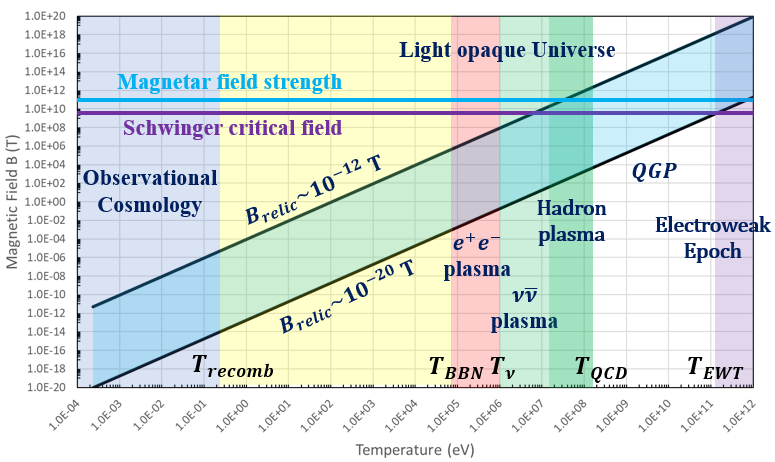
\includegraphics[scale=0.75]{relic_plot.PNG}
    \label{fig1}
    \caption{Qualitative value of the primordial magnetic field over the evolutionary lifespan of the universe. As magnetic flux is conserved over comoving surfaces, the primordial relic field is expected to dilute as $\approx1/a(t)^{2}$ meaning the contemporary small bound values of $5\times10^{-12}\ \mathrm{T}>B_{relic}>10^{-20}\ \mathrm{T}$ may have once represented large magnetic fields in the early universe. This is relic magnetic field would then be generated by the last phase of significant magnetization in the early universe. This figure is meant to be illustrative and it is unlikely the magnetization of the universe would proceed unhindered and unaltered into the ultra-dense plasma phases of the early universe. The values of the Schwinger critical field and the upper bound of surface magnetar field strength are included for scale.}
    \centering
\end{figure}
This reveals that only the mass contribution is dynamical over cosmological time. For any given eigen-state, the mass term increases driving the state into the non-relativistic limit while the momenta and magnetic contributions are frozen by initial conditions. We can specifically introduce a dimensionless magnetic scale which is frozen in the homogenous case as
\begin{alignat}{1}
    \label{Bo} b_{0}\equiv\frac{qB\hbar c^{2}}{(k_{B}T)^{2}}\,,
\end{alignat}
written explicitly in full SI units. If the origin of deep space extra-galactic magnetic fields are relic fields from the early universe, which today are expected to exist between $5\times10^{-12}\ \mathrm{T}>B_{relic}>10^{-20}\ \mathrm{T}$, then the value of the magnetic scale is between
\begin{alignat}{1}
    \label{BoScale} 5.5\times10^{-5}>b_{0}>1.1\times10^{-11}\,.
\end{alignat}
This should remain constant in the universe at-large up to the last epoch the universe was sufficiently magnetized to disturb this value. As the electron-proton plasma which generated the CMB was relatively dilute over its duration, it was unlikely sufficiently magnetized to significantly alter this value over extra-galactic scales. Rather, the best candidate plasma to have been sufficiently magnetized and dense to have set the relic field magnetic scale would have been the electron-positron plasma which existed during the duration of Big Bang Nucleosynthesis (BBN).

Higher order non-minimal magnetic contributions like $\approx\mu_{B}^{2}B^{2}/T^{2}$ are even more surpressed over cosmological time which drives the system into minimal electromagnetic coupling with the exception of the anomalous magnetic moment. It is interesting that cosmological expansion serves to \lq\lq smooth out\rq\rq\ the features of more complex BSM electrodynmaic features erasing them from a statistical perspective.

\section{Partition Function}\label{sec:Stats}
\noindent Now that we've obtained the energy eigenvalues of the KGP particle, we can work towards evaluating the grand partition function of the system and ultimately the magnetic properties of the magnetized KGP Fermi gas. In addition to considering polarization, there are also the positive and negative energy states. The grand partition function for the relativistic Fermi-Dirac ensemble is given by the standard definition
\begin{alignat}{1}
    \label{PartFunc} \ln\left(\mathcal{Z}_{L}\right)=\sum_{\alpha}\ln\left(1+z_{\sigma}\exp(-X_{s})\right)\,,
\end{alignat}
where we are summing over all possible quantum numbers $\alpha = \{p_{z},n,s,\sigma,\tilde{g}\}$. The summation over $\tilde{g}$ represents the occupancy of Landau states which are matched to the available phase space within $\Delta p_{x}\Delta p_{y}$. The fugacity $z_{\sigma}$ is defined as
\begin{alignat}{1}
    \label{Fugacity} z_{\sigma}=\exp\left(\sigma\eta\right)\,,
\end{alignat}
where $\eta$ is the chemical potential of the species and $\sigma\in\pm1$ denotes between particles and antiparticles. The chemical potential $\eta$ is an increasing function of the number of particles present within a given volume and fixed by the particle number
\begin{alignat}{1}
  \label{Number} N=\sum_{\alpha}\langle n_{\alpha}\rangle=\sum_{\alpha}\frac{1}{\exp(X_{s})z_{\sigma}^{-1}+1}\,.
\end{alignat}
If we consider the Landau energies to represent the transverse momentum $p_{T}^{2}=p_{x}^{2}+p_{y}^{2}$ of the system, then the relationship that defines $\tilde{g}$ is given by
\begin{alignat}{1}
    \label{PhaseSpace} \frac{L^{2}}{(2\pi)^{2}}\Delta p_{x}\Delta p_{y}=\frac{qBL^{2}}{2\pi}\Delta n\,,\indent \tilde{g}=\frac{eBL^{2}}{2\pi}\,.
\end{alignat}
The summation over the continous $p_{z}$ can be replaced with an integration
\begin{alignat}{1}
    \label{pzInt} \sum_{p_{z}}\rightarrow\frac{L}{2\pi}\int^{+\infty}_{-\infty}dp_{z}\,,
\end{alignat}
where $L$ defines the boundary length of our considered volume. The partition function \req{PartFunc} can be then rewritten as
\begin{alignat}{1}
    \label{PartFuncOne} \ln\left(\mathcal{Z}_{L}\right)=\sum_{\sigma}^{\pm1}\sum_{s}^{\pm1/2}\frac{2eBL^{3}}{(2\pi)^{2}}\int^{+\infty}_{0}dp_{z}\sum_{n=0}^{\infty}\ln\left(1+z_{\sigma}\exp(-X_{s})\right)\,.
\end{alignat}
We note that the partition function can be broken into four quantum gasses: Particles and antiparticles, and spin aligned and antialigned. This can be represented by separate partition functions $\ln\left(\mathcal{Z}^{\sigma}_{s}\right)$ where
\begin{alignat}{1}
    \label{FourGasses} \ln\left(\mathcal{Z}_{L}\right)=\sum_{\sigma,s}\ln\left(\mathcal{Z}^{\sigma}_{s}\right)\,,
\end{alignat}
For KGP particles, the anomalous moment (a) breaks the degeneracy between Landau levels of opposite alignment and (b) depending on the size of the anomaly, flips the sign of the magnetic contribution to the energy for certain eccentric states. For $0<a<2$ the aligned ground state is uniquely separated from the rest of the states while for $2<a<4$ the aligned ground state and first excited state are uniquely separated. The pattern of unique eccentric states continues for further extreme values of anomalous moment. While we consider the $g$-factor to be the immutable description of magnetic moment, it is useful in the case of Landau levels to consider the anomaly $a$ as from the energies given in eq.~\eqref{LANeq02}, $g$ always is linearly added or subtracted from the Landau quantum number which are integers.

Degeneracy is restored for values of the anomalous parameter given in eq.~\eqref{LANeq04}. While generating a large number of eccentric states from large anomalous moment may be of theoretical interest, it is of practical interest to consider particles like the proton or electron where only the ground state is uniquely disturbed. Due to the properties of logs, the overall partition function will be sum of the partition function of each species, which allows us to consider each species separately. The next step is to replace the sum over $n$ Landau levels and replace it with an integration using the Euler-Maclaurin integration formula. The Euler-Maclaurin formula is given by
\begin{alignat}{1}
    \label{EulerM} \sum^{b}_{n=a}f(n)-\int^{b}_{a}f(x)dx = \frac{1}{2}\left(f(b)+f(a)\right)+\sum_{i=1}^{k}\frac{b_{2i}}{(2i)!}\left(f^{(2i-1)}(b)-f^{(2i-1)}(a)\right)+R(k)\,,
\end{alignat}
where $b_{n}$ are the Bernoulli numbers and $R(k)$ is the error remainder defined by integrals over Bernoulli polynomials. The integer $k$ is chosen for the level of approximation that is desired. Using \req{EulerM} allows us to convert the sum over $n$ quantum numbers in \req{PartFuncOne} into an integral. We define
\begin{alignat}{1}
    \label{Func} f(p_{z},n,s,\sigma)=\ln\left(1+z_{\sigma}\exp(-X_{s})\right)\,,
\end{alignat}
The result for $k=1$ is
\begin{alignat}{1}
    \label{PartFuncTwo} \ln\left(\mathcal{Z}_{s}^{\sigma}\right)=\frac{2eBL^{3}}{(2\pi)^{2}}\int_{0}^{+\infty}dp_{z}\left(\int_{0}^{+\infty}dn f(n) + \frac{1}{2}f(0) + \frac{1}{12}\frac{\partial f(n)}{\partial n}\bigg\rvert_{n=0} + R(1)\right)
\end{alignat}
It is to be recognized that the first term in expression \req{PartFuncTwo} is merely the free particle fermion partition function with a rescaled mass $m_{s}$. This then allows us to achieve our goal of a \lq\lq separated\rq\rq\ partition function which explicitly reveals the particle portion of the phase-phase and the spin portions as different contributions. This separation is however not fully independant as the rescaled mass $m_{s}$ is intrinsically a function of the spin alignment. It will be demonstrated further below that the free-like portion is the relativistic equivalent of the Hamiltonian modified by $E_{M}=-\bb{\mu}\cdot\bb{B}$ dipole energies. We introduce the dimensionless variables
\begin{alignat}{1}
    \label{Unitless} a_{s}=\frac{m_{s}}{T}\,,\indent y_{s}=\frac{p_{z}}{m_{s}}\,,\indent u_{s}=\frac{2qB}{m_{s}^{2}}n\,,
\end{alignat}
which allows us to express \req{Boltz} as
\begin{alignat}{1}
    \label{UnitlessBoltz} X_{s}(y_{s},u_{s})=a_{s}\sqrt{1+y_{s}^{2}+u_{s}}\,.
\end{alignat}
Via substitution of dimensionless variables, and some rearrangment, we can write the magnetized partition function in terms of free fermion partition functions of differing masses, yielding,
\begin{alignat}{1}
    \label{Equality} \ln\left(\mathcal{Z}^{\sigma}_{s}\right) = \ln\left(\mathcal{Z}^{\sigma}_{F}\right)|_{m_{s}} + \frac{2eBL^{3}}{(2\pi)^{2}}m_{s}\int_{0}^{+\infty}dy\left(\frac{1}{2}f(0) + \frac{1}{12}\frac{\partial f(n)}{\partial n}\bigg\rvert_{n=0} + R(1)\right)\,,
\end{alignat}
where we have dropped the spin subscript from the dimensionless z-momentum $y$ as it is does not impact the limits of integration. The free-like portion of the partition function is given by
\begin{alignat}{1}
    \label{Freelike} \ln\left(\mathcal{Z}^{\sigma}_{F}\right)|_{m_{s}}=\frac{L^{3}}{(2\pi)^{3}}\int^{+\infty}_{-\infty}d\bb{p}^{3}\ln\left(1+z_{\sigma}\exp(-X^{s}_{F})\right)\,,\\
    \label{FreelikeHam} X^{s}_{F} = a_{s}\sqrt{1+y^{2}}
\end{alignat}
In dimensionless units we can represent \req{Freelike} as
\begin{alignat}{1}
    \label{FreelikeAlt} \ln\left(\mathcal{Z}^{\sigma}_{F}\right)|_{m_{s}}=\frac{L^{3}}{(2\pi)^{2}}m_{s}^{3}\int^{+\infty}_{-\infty}dy\left[y^{2}\ln\left(1+z_{\sigma}\exp(-X^{s}_{F})\right)\right]\,,
\end{alignat}
Integrating by parts, we arrive at
\begin{alignat}{1}
    \label{FreelikeParts} \ln\left(\mathcal{Z}^{\sigma}_{F}\right)|_{m_{s}}=\frac{1}{3}\frac{L^{3}}{(2\pi)^{2}}m_{s}^{4}\left(\frac{m_{s}}{T}\right)\int^{+\infty}_{-\infty}dy\left[\frac{y^{4}}{\epsilon}F[X_{s},\sigma]\right]\,,\\
    \label{EigenE} \epsilon = a_{s}\sqrt{1+y^{2}}\,,\\
    \label{FermD} F[X_{s},\sigma] = \frac{1}{\exp(X_{s})z_{\sigma}^{-1}+1}\,,
\end{alignat}
where $\epsilon$ is the free eigen-energy and $F$ is the Fermi distribution. By introducing a change of variables of $y=\sinh(t)$ this simplifies to
\begin{alignat}{1}
    \label{FreelikeFinal} \ln\left(\mathcal{Z}^{\sigma}_{F}\right)|_{m_{s}}=\frac{1}{3}\frac{L^{3}}{(2\pi)^{2}}m_{s}^{4}\left(\frac{m_{s}}{T}\right)\int^{+\infty}_{-\infty}dt\left[\frac{\sinh(t)^{4}}{\exp(a_{s}\cosh(t))z_{\sigma}^{-1}+1}\right]\,,
\end{alignat}
This integrand is well behaved and has a finite integration value within the restriction that $m_{s}$ remains physical. The magnetization of this term, defined by \req{Mag}, is found to be
\begin{alignat}{1}
    \label{FreelikeMag} M_{F}^{\sigma}=\frac{T}{V}\frac{\partial m_{s}}{\partial B}\frac{\partial}{\partial m_{s}}\ln(\mathcal{Z}_{F}^{\sigma})\,\,,
\end{alignat}


\end{document}
